\chapter{传输层}\label{CN05}

\section{端口、连接与数据边界}\label{CN05-endpoints}

传输层为不同主机的进程端点提供逻辑通信，完成复用与分用。端口16 bit，TCP与UDP端口空间独立；熟知端口0～1023、登记1024～49151、动态/私有49152～65535。端口标识应用端点，具体进程可管理多个套接字。

TCP连接由源IP、源端口、目的IP、目的端口四元组区分，服务器同一服务端口可对应多个客户。UDP基本分用按目的端口等本地端点信息，实际绑定或连接方式可再限定远端。

\par\medskip\Needspace{4\baselineskip}\noindent\hypertarget{CN05-E01}{}\label{CN05-E01}\textbf{例 5-1}\par\nobreak\smallskip

UDP协议实现分用时所依据的头部字段是（　）。

A. 源端口号　B. 目的端口号　C. 长度　D. 校验和

\par\smallskip
\begin{wideblock}
{\fontsize{9.3}{12}\selectfont\setlength{\tabcolsep}{2.5pt}\setlength{\LTleft}{0pt}\setlength{\LTright}{0pt}
\begin{longtable}{@{}>{\raggedright\arraybackslash}p{\dimexpr0.20986\linewidth-2\tabcolsep\relax}>{\raggedright\arraybackslash}p{\dimexpr0.41123\linewidth-2\tabcolsep\relax}>{\raggedright\arraybackslash}p{\dimexpr0.37891\linewidth-2\tabcolsep\relax}@{}}
\toprule
比较项 & UDP & TCP \\

\midrule\endfirsthead\toprule
比较项 & UDP & TCP \\

\midrule\endhead\bottomrule\endfoot
服务 & 无连接、尽最大努力；可按下层能力单播/组播/广播 & 面向连接、一对一、全双工可靠有序字节流 \\

应用边界 & 保留每个报文边界 & 不保留写入边界，应用自行定界 \\

首部 & 固定8 B & 20～60 B \\

可靠性与控制 & 无自身确认重传、顺序恢复或拥塞窗口 & 序号、累计ACK、重传、接收窗口与拥塞控制 \\

\end{longtable}}
\end{wideblock}
\par\smallskip

TCP发送缓冲保留未确认字节以便重传；接收缓冲可存失序字节，按序交付。应用读取后释放接收空间。MSS限制单段应用数据上限，分段可跨越应用写入边界；普通MTU1500、IP/TCP各20 B时简单模型MSS1460 B，选项或路径改变须重算。

\section{UDP长度与反码检验和}\label{CN05-udp-checksum}

\begin{figure}[H]
\centering
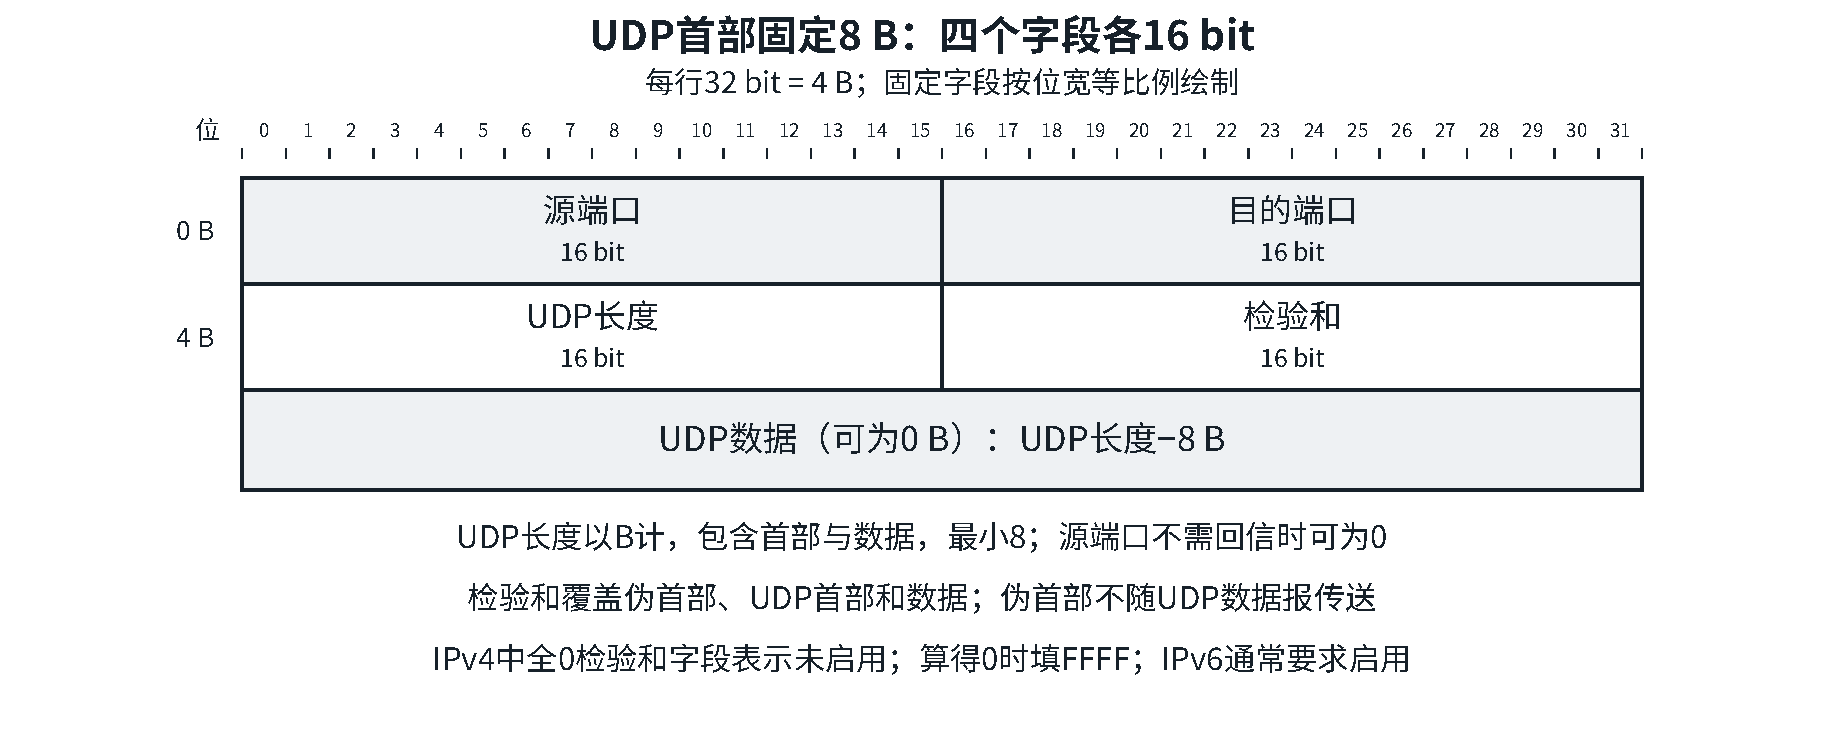
\includegraphics[width=\linewidth,height=108mm,keepaspectratio]{figures/CN18_udp_header.pdf}
\caption{UDP四字段各16 bit}\label{cn-fig-udp-format}
\end{figure}

UDP源端口供回复，不需回复时可为0；目的端口分用；长度计首部加数据，最小8 B；校验和检错。普通IPv4首部20 B时UDP应用数据最大\(65535-20-8=65507\) B。UDP不自行拆成多个UDP报文，承载IP可分片，目的IP重组后交UDP。

发送端校验和置0，按16 bit分组求反码和：进位回卷到最低位，直到无进位，再按位取反；奇数字节末尾补0仅参与计算。接收端连同校验和求反码和应为\texttt{FFFF}，仍存在抵消漏检。

\par\smallskip
\begin{wideblock}
{\fontsize{9.3}{12}\selectfont\setlength{\tabcolsep}{2.5pt}\setlength{\LTleft}{0pt}\setlength{\LTright}{0pt}
\begin{longtable}{@{}>{\raggedright\arraybackslash}p{\dimexpr0.18828\linewidth-2\tabcolsep\relax}>{\raggedright\arraybackslash}p{\dimexpr0.30290\linewidth-2\tabcolsep\relax}>{\raggedright\arraybackslash}p{\dimexpr0.50883\linewidth-2\tabcolsep\relax}@{}}
\toprule
检验 & 覆盖内容 & 零字段规则 \\

\midrule\endfirsthead\toprule
检验 & 覆盖内容 & 零字段规则 \\

\midrule\endhead\bottomrule\endfoot
IPv4首部 & IP首部、选项、填充 & 无关闭校验语义 \\

UDP & 伪首部、UDP首部与数据 & IPv4可用全0表示未启用；算得0传全1；普通IPv6 UDP通常必须启用 \\

TCP & 伪首部、TCP首部与数据 & 无以全0关闭校验约定 \\

\end{longtable}}
\end{wideblock}
\par\smallskip

IPv4伪首部12 B：源IP、目的IP、0、协议号、传输层长度；UDP协议17，TCP协议6。伪首部及求和补0不在线上传输，不计入应用长度。NAT改IP会影响伪首部，启用的传输校验需更新；普通TTL变化只影响IPv4首部检验和。

\par\medskip\Needspace{4\baselineskip}\noindent\hypertarget{CN05-E02}{}\label{CN05-E02}\textbf{例 5-2}\par\nobreak\smallskip

若UDP协议在计算校验和过程中，计算得到中间结果为 \texttt{1011 1001 1011 0110} 时，还需要加上最后一个16位数 \texttt{0110 0101 1100 0101}，则最终计算得到的校验和是（　）。

A. \texttt{0001 1111 0111 1011}

B. \texttt{0001 1111 0111 1100}

C. \texttt{1110 0000 1000 0011}

D. \texttt{1110 0000 1000 0100}

\section{TCP首部、序号与累计确认}\label{CN05-tcp-header}

\begin{figure}[H]
\centering
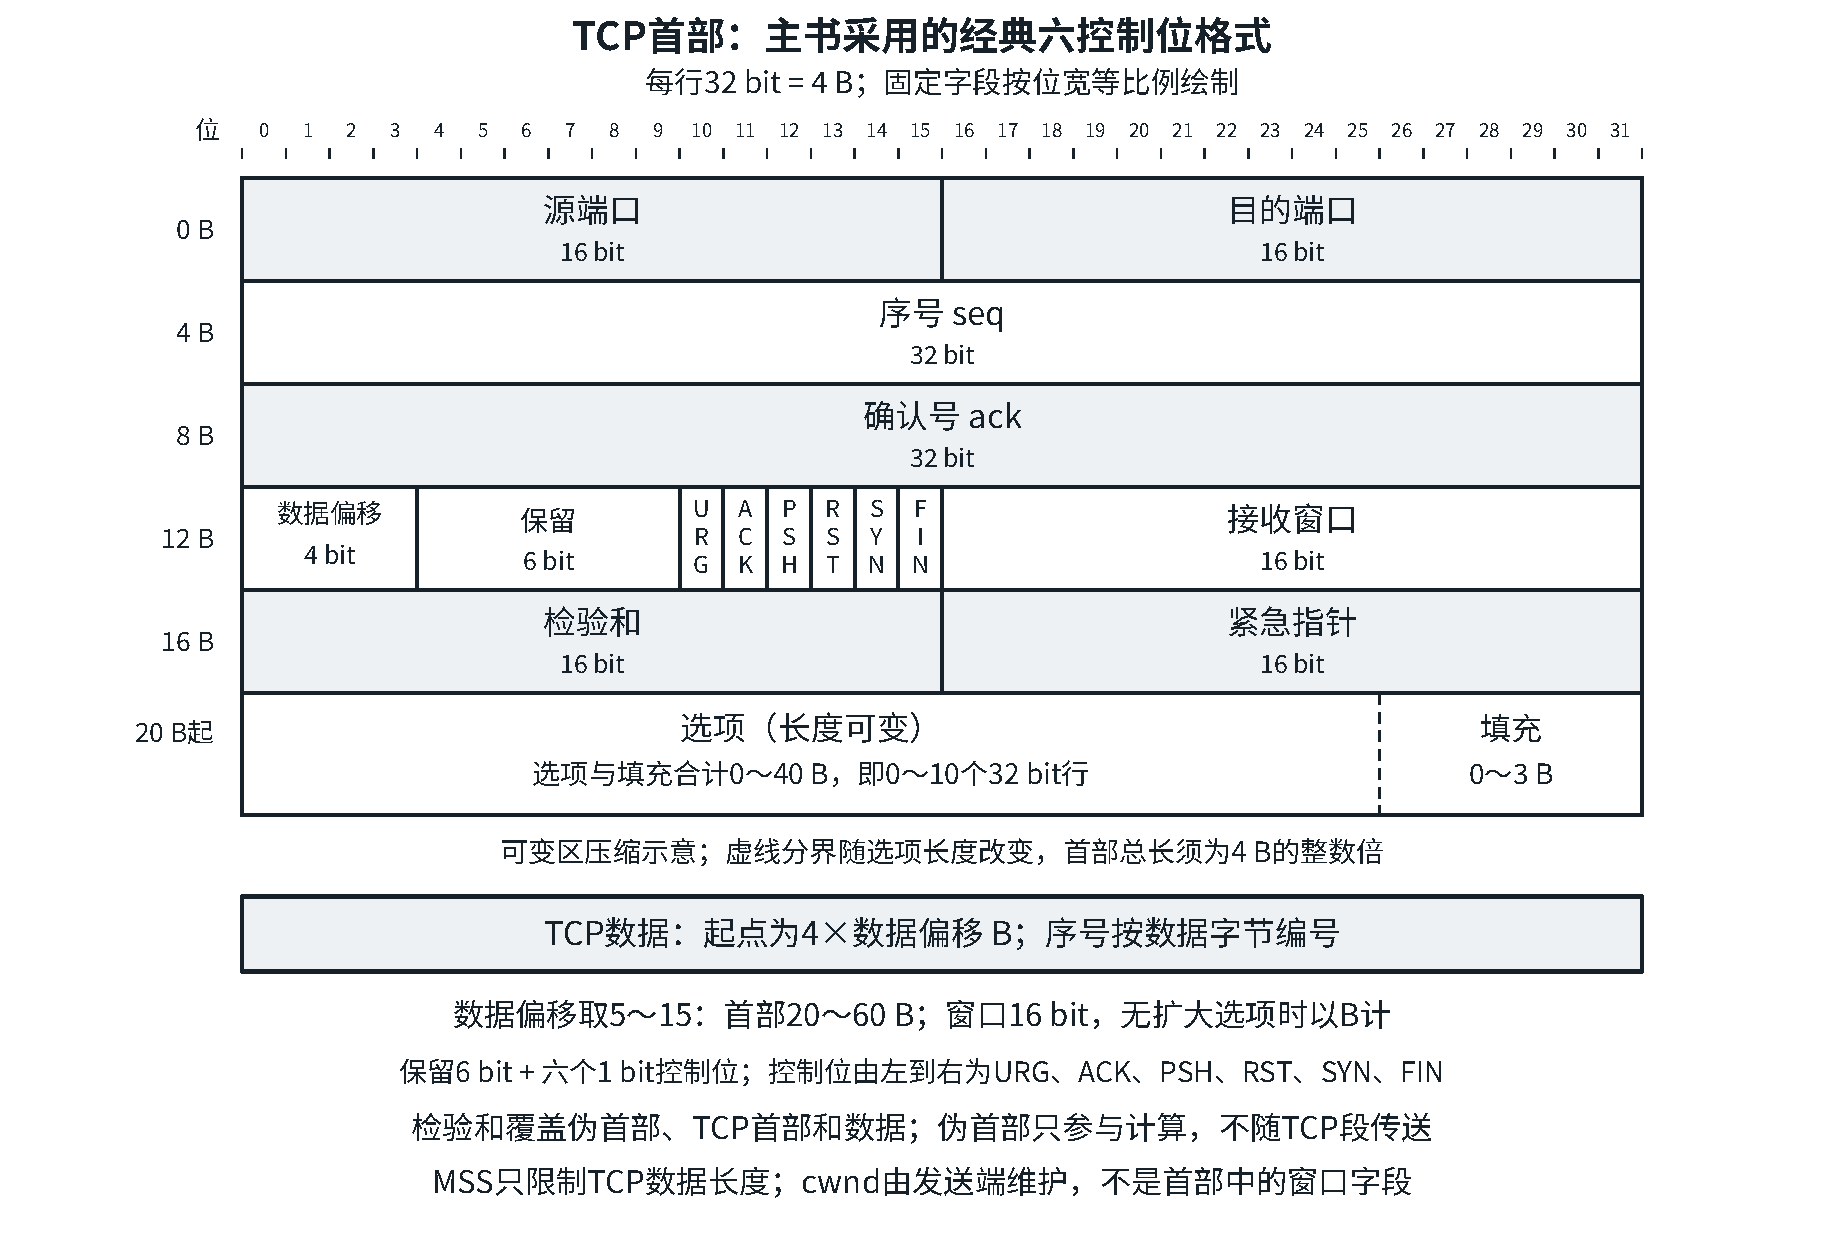
\includegraphics[width=\linewidth,height=108mm,keepaspectratio]{figures/CN17_tcp_header.pdf}
\caption{教材TCP固定首部及六控制位}\label{cn-fig-tcp-format}
\end{figure}

源/目的端口各16 bit，seq/ack各32 bit；数据偏移4 bit、单位4 B，表示TCP首长，取5～15；接收窗口16 bit，未扩大时以B计、最大65535；检验和和紧急指针各16 bit，选项填充至4 B对齐。题图采用教材六控制位口径，扩展位按题设解释。

未分片或已重组的普通IPv4仅承载一个TCP段时：

\[L_{TCP数据}=IP总长-4IHL-4\times TCP数据偏移.\]

\par\smallskip
{\fontsize{9.3}{12}\selectfont\setlength{\tabcolsep}{2.5pt}\setlength{\LTleft}{0pt}\setlength{\LTright}{0pt}
\begin{longtable}{@{}>{\raggedright\arraybackslash}p{\dimexpr0.26748\linewidth-2\tabcolsep\relax}>{\raggedright\arraybackslash}p{\dimexpr0.73252\linewidth-2\tabcolsep\relax}@{}}
\toprule
控制位 & 含义 \\

\midrule\endfirsthead\toprule
控制位 & 含义 \\

\midrule\endhead\bottomrule\endfoot
SYN & 同步初始序号，占1个序号 \\

ACK & 为1时确认号有效；纯ACK不占序号 \\

FIN & 本方向不再发送，占1个序号 \\

RST & 复位、拒绝不适当连接或段 \\

PSH & 请求及时向应用交付 \\

URG & 紧急指针有效；指针相对seq给出紧急数据边界，按教材前置紧急数据模型理解 \\

\end{longtable}}
\par\smallskip

TCP按字节编号，序号模\(2^{32}\)；无回绕时，seq=\(s\)、数据长\(L\)覆盖\(s\)～\(s+L-1\)，下一号\(s+L\)。ack=\(a\)累计确认连续收到至\(a-1\)，期望\(a\)。两方向序号空间独立，捎带段中的seq和ack分别记账。SYN序号\(x\)后首数据\(x+1\)；FIN后确认号也加1，这些消耗不计为应用字节。

\par\medskip\Needspace{4\baselineskip}\noindent\hypertarget{CN05-E03}{}\label{CN05-E03}\textbf{例 5-3}\par\nobreak\smallskip

主机甲与主机乙之间已建立一个TCP连接，甲向乙发送了两个连续TCP段，分别包含300 B和500 B有效载荷，第一个段的序列号为200，乙正确接收到两个段后，发送给甲的确认序列号是（　）。

A. 500　B. 700　C. 800　D. 1000

\section{三次握手、半关闭与TIME-WAIT}\label{CN05-connection}

\par\smallskip
\begin{wideblock}
{\fontsize{9.3}{12}\selectfont\setlength{\tabcolsep}{2.5pt}\setlength{\LTleft}{0pt}\setlength{\LTright}{0pt}
\begin{longtable}{@{}>{\raggedright\arraybackslash}p{\dimexpr0.39931\linewidth-2\tabcolsep\relax}>{\raggedright\arraybackslash}p{\dimexpr0.29652\linewidth-2\tabcolsep\relax}>{\raggedright\arraybackslash}p{\dimexpr0.30417\linewidth-2\tabcolsep\relax}@{}}
\toprule
事件 & 客户状态/动作 & 服务器状态/动作 \\

\midrule\endfirsthead\toprule
事件 & 客户状态/动作 & 服务器状态/动作 \\

\midrule\endhead\bottomrule\endfoot
客户发SYN，seq=\(x\) & SYN-SENT & LISTEN等待 \\

服务器收SYN并回SYN+ACK，seq=\(y\)、ack=\(x+1\) & 等待回复 & SYN-RECEIVED \\

客户收到并回ACK，seq=\(x+1\)、ack=\(y+1\) & ESTABLISHED，可带数据 & 收到此ACK后ESTABLISHED \\

\end{longtable}}
\end{wideblock}
\par\smallskip

第三次握手确认服务器初始序号，避免服务器仅凭迟到旧SYN就长期保留无效连接。

\begin{figure}[H]
\centering
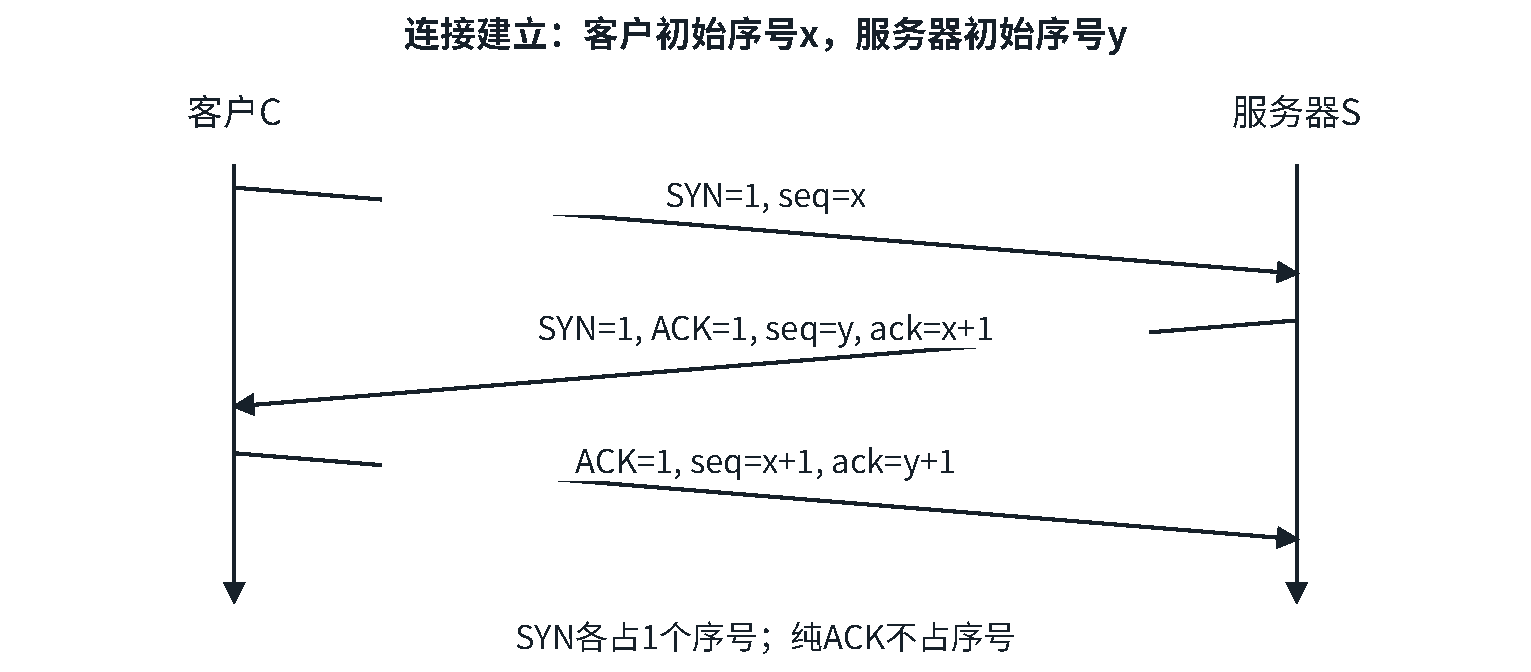
\includegraphics[width=\linewidth,height=108mm,keepaspectratio]{figures/CN09_tcp_handshake.pdf}
\caption{两个方向各同步一个初始序号}\label{cn-fig-handshake}
\end{figure}

主动端发FIN进入FIN-WAIT-1；收其ACK到FIN-WAIT-2；收对方FIN并回ACK到TIME-WAIT；2MSL后CLOSED。被动端收FIN回ACK到CLOSE-WAIT，本方向仍可发数据；应用关闭后发FIN到LAST-ACK，收确认后CLOSED。ACK与FIN可合并；同时关闭可经CLOSING，按事件次序判断。

TIME-WAIT的2MSL使最后ACK丢失时仍可响应重传FIN，并让旧连接报文消散。两端关闭时间分别按本端状态进入事件计算。

\par\medskip\Needspace{4\baselineskip}\noindent\hypertarget{CN05-E04}{}\label{CN05-E04}\textbf{例 5-4}\par\nobreak\smallskip

假设客户C和服务器S已建立TCP连接，RTT=50 ms，最长报文段寿命MSL=800 ms，数据传输结束后C主动请求断开连接。若从C主动向S发出FIN段时刻算起，则C和S进入CLOSED状态所需的时间至少分别是（　）。

A. 850 ms，50 ms　B. 1650 ms，50 ms

C. 850 ms，75 ms　D. 1650 ms，75 ms

\section{重传、重复ACK与RTT估计}\label{CN05-retransmission}

失序到达时累计ACK保持缺口首字节；接收方可缓存，SACK另报已收分块而不改变累计ACK。发送端保留未确认字节，超时重传相关未确认数据。经典快重传在3个重复ACK时触发，不计最初推进确认号的正常ACK。

例如622到达返回ACK623，623丢失；624、625、626依次到达分别产生重复ACK1、2、3，第三份才触发快重传。若已缓存624～626，补齐623后ACK可推进至627。

\begin{figure}[H]
\centering
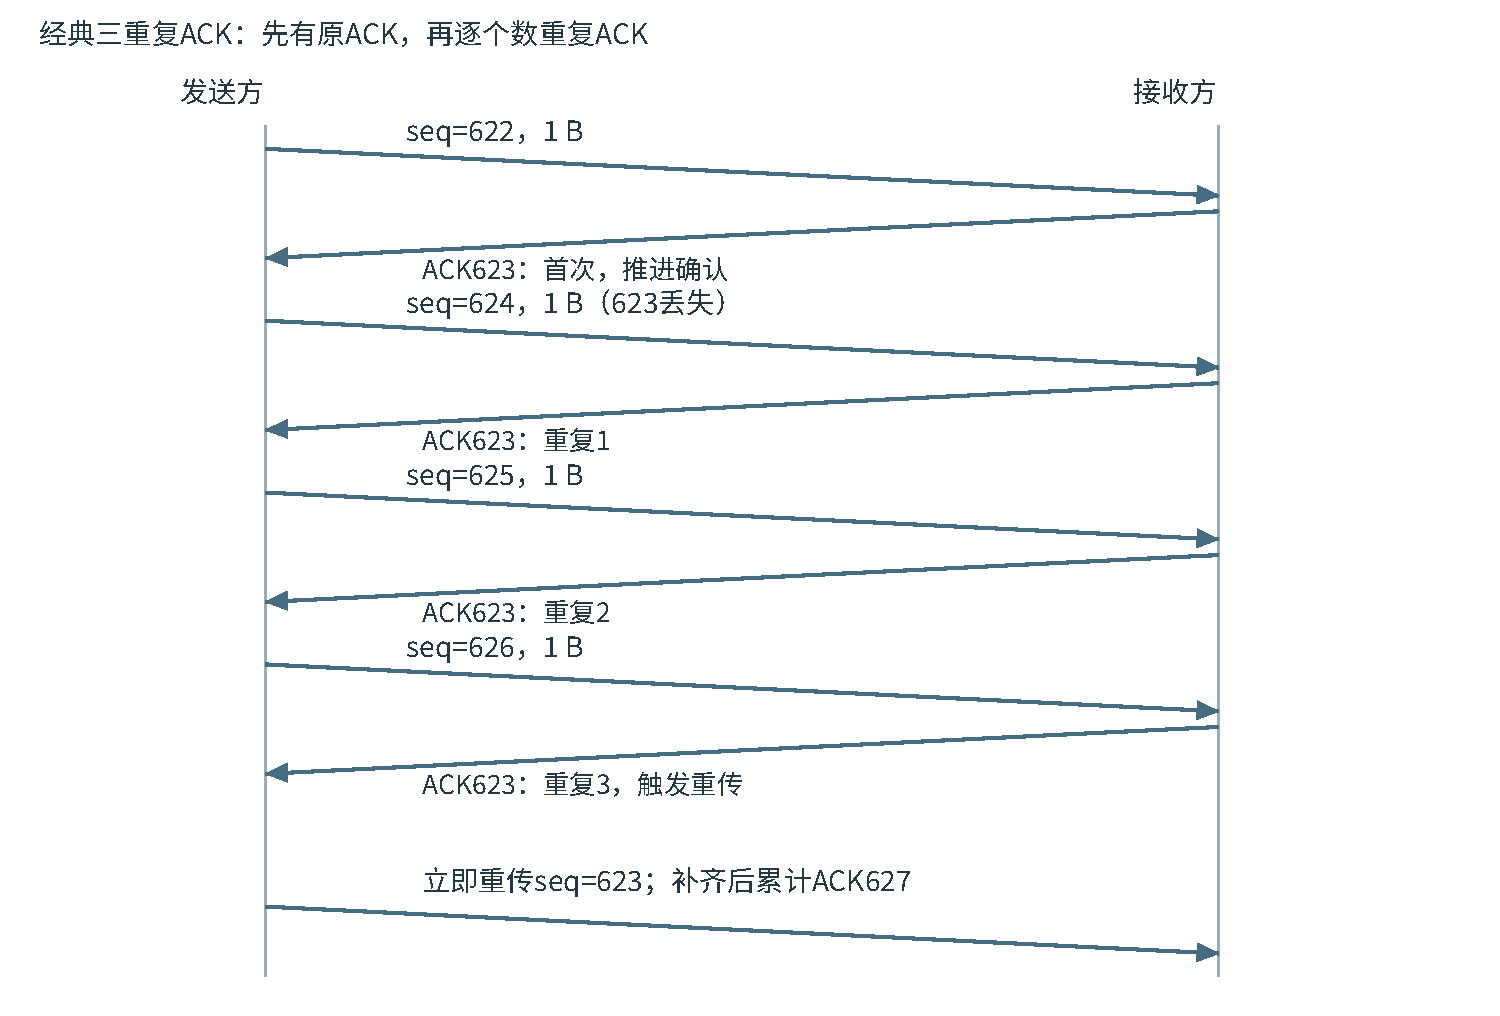
\includegraphics[width=\linewidth,height=108mm,keepaspectratio]{figures/CN_course_duplicate_acks.pdf}
\caption{正常ACK与三次重复ACK分别计数}\label{cn-course-duplicate-acks}
\end{figure}

\[SRTT\leftarrow(1-\alpha)SRTT+\alpha RTT_{sample}.\]

RTO结合平滑RTT及偏差估计，题给\(RTO=\beta SRTT\)时按其简化式；超时后RTO退避。Karn原则排除有重传歧义的RTT样本。旧SRTT100 ms、\(\alpha=1/8\)、有效样本140 ms，则新值105 ms。

\section{接收窗口、拥塞窗口与可新发额度}\label{CN05-windows}

rwnd由接收方依据当前接收能力通告，cwnd由发送方依据网络反馈维护。ack=\(a\)、rwnd=\(w\)允许范围\(a\)～\(a+w-1\)；首部窗口字段反映本段发送者的接收能力。扩大选项在握手协商，未给则不自行放大。

当最新ACK与窗口左沿一致，已发未确认字节量\(F\)：

\[W=\min(cwnd,rwnd),\qquad A=\max(0,W-F).\]

\(W\)为总发送额度，\(A\)为还可新发；已在途量继续占额度，窗口缩小不要求撤回已发数据。复杂窗口更新按实际字节区间和有效右边界记录。

零窗口暂停普通数据发送，持续计时器触发零窗口探测，防止窗口重开通知丢失造成永久等待。它与重传、保活、TIME-WAIT计时器分别处理不同事件。

接收缓存8 B且应用不读，从seq600开始，依次收到600～602、603～604、605～606、607：ACK/rwnd为603/5、605/3、607/1、608/0；应用读走8 B后为608/8，确认号保持。

\par\medskip\Needspace{4\baselineskip}\noindent\hypertarget{CN05-E06}{}\label{CN05-E06}\textbf{例 5-5}\par\nobreak\smallskip

主机甲通过TCP向主机乙发送数据的部分过程如下图。seq为序号，ack\_seq为确认序号，rcvwnd为接收窗口。甲在 \(t_0\) 的拥塞窗口和发送窗口均为2000 B，拥塞控制阈值为8000 B，MSS=1000 B，甲始终以MSS发送TCP段。若甲在 \(t_1\) 收到图示确认段，则未收到新的确认之前，还可以继续发送的TCP段数是（　）。

\begin{figure}[H]
\centering
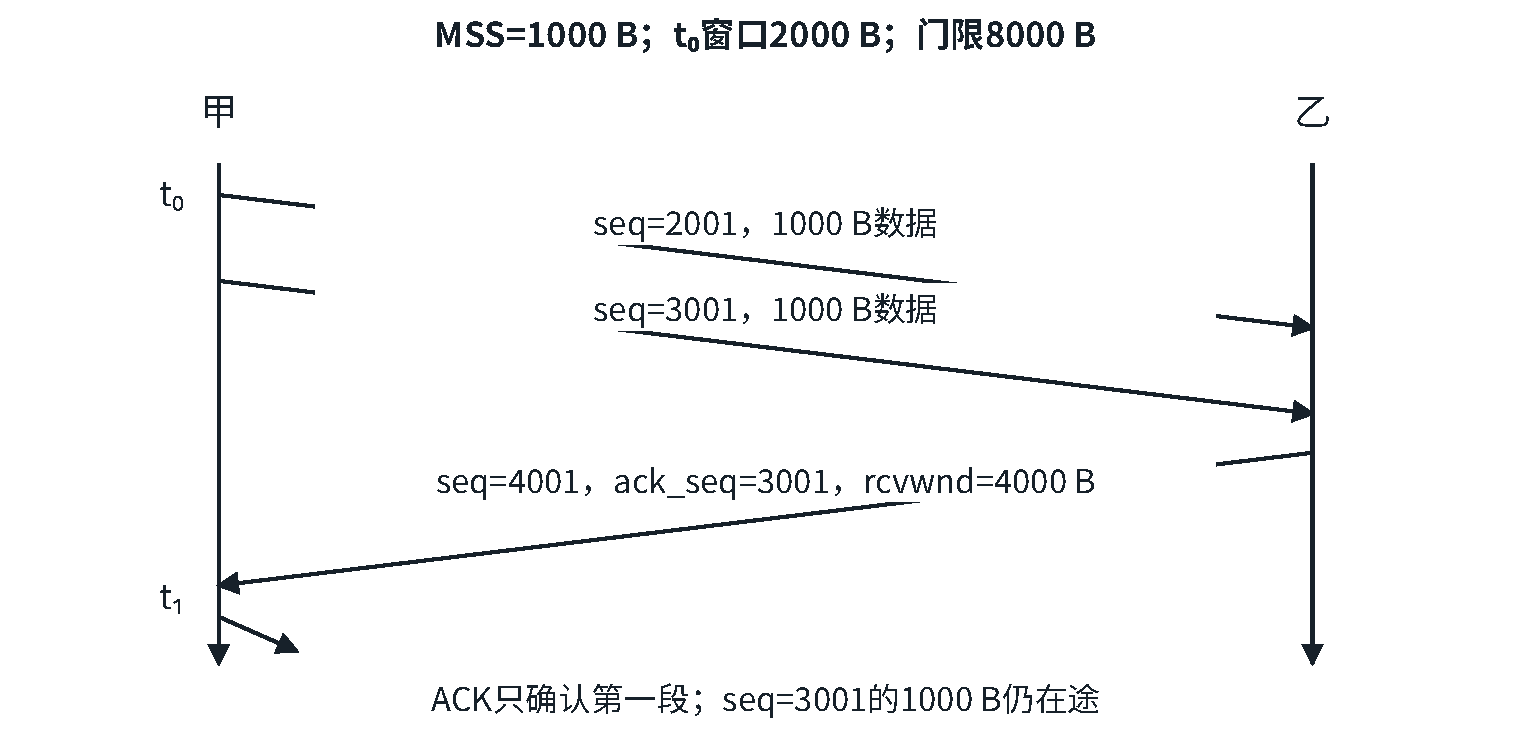
\includegraphics[width=\linewidth,height=108mm,keepaspectratio]{figures/CN10_tcp_window_2025.pdf}
\caption{原题数据：第二个数据段仍未被ack\_seq=3001确认}\label{cn-fig-tcp-window}
\end{figure}

A. 2　B. 3　C. 4　D. 5

\section{慢开始、拥塞避免与Reno恢复}\label{CN05-congestion}

以下为教材逐段确认、持续有数据、无其他限制的简化模型，初始窗口按题设，常用1 MSS。慢开始每个新数据ACK增加约1 MSS，完整一轮约翻倍；达到ssthresh后拥塞避免，每RTT约增1 MSS。延迟ACK、应用受限、rwnd受限会改变轨迹，轮次须注明发送前或确认后记录。

\par\smallskip
\begin{wideblock}
{\fontsize{9.3}{12}\selectfont\setlength{\tabcolsep}{2.5pt}\setlength{\LTleft}{0pt}\setlength{\LTright}{0pt}
\begin{longtable}{@{}>{\raggedright\arraybackslash}p{\dimexpr0.23305\linewidth-2\tabcolsep\relax}>{\raggedright\arraybackslash}p{\dimexpr0.28991\linewidth-2\tabcolsep\relax}>{\raggedright\arraybackslash}p{\dimexpr0.47704\linewidth-2\tabcolsep\relax}@{}}
\toprule
事件 & ssthresh & cwnd及后续 \\

\midrule\endfirsthead\toprule
事件 & ssthresh & cwnd及后续 \\

\midrule\endhead\bottomrule\endfoot
超时 & 教材常取丢包时cwnd一半 & 回1 MSS，再慢开始 \\

Reno三重复ACK & 教材常取原窗口一半 & 快重传，快恢复临时为门限+3 MSS；新ACK确认缺失数据后回门限，转拥塞避免 \\

Tahoe三重复ACK & 减半门限 & 回1 MSS并慢开始 \\

\end{longtable}}
\end{wideblock}
\par\smallskip

课件稳定轮次图通常记录快恢复完成后的cwnd=ssthresh，恢复中临时+3另算。规范实现设门限还参考在途量，题目明确模型优先。

初始1、门限8，未受其他限制时轮次1、2、4、8、9、10\ldots\ldots；若在12超时，门限6，后续1、2、4、6、7\ldots\ldots。

\par\medskip\Needspace{4\baselineskip}\noindent\hypertarget{CN05-E05}{}\label{CN05-E05}\textbf{例 5-6}\par\nobreak\smallskip

若主机甲与主机乙已建立TCP连接，MSS为1 KB，RTT为2 ms，则在不出现拥塞的前提下，拥塞窗口从8 KB增长到32 KB所需的最长时间是（　）。

A. 4 ms　B. 8 ms　C. 24 ms　D. 48 ms

\par\medskip\Needspace{4\baselineskip}\noindent\hypertarget{CN05-E07}{}\label{CN05-E07}\textbf{例 5-7}\par\nobreak\smallskip

主机甲和乙已建立TCP连接，甲始终以MSS=1 KB大小的段发送数据，并一直有数据发送；乙每收到一个数据段都会发出一个接收窗口为10 KB的确认段。若甲在 \(t\) 时刻发生超时时拥塞窗口为8 KB，则从 \(t\) 起不再发生超时的情况下，经过10个RTT后，甲的发送窗口是（　）。

A. 10 KB　B. 12 KB　C. 14 KB　D. 15 KB

\section{TCP字段与接收缓存综合计算}\label{CN05-integrated}

按“IP长度和首长\ensuremath{\to}TCP起点与数据偏移\ensuremath{\to}控制位\ensuremath{\to}两方向seq/ack\ensuremath{\to}窗口”解码。以太网填充比较整个IP长度与最小数据区，填充不占IP总长或TCP序号。TTL差计路由器跳数，交换机不减TTL；有NAT时结合IP标识和TCP字段识别对应分组。

\par\medskip\Needspace{4\baselineskip}\noindent\hypertarget{CN05-E08}{}\label{CN05-E08}\textbf{例 5-8}\par\nobreak\smallskip

主机H通过快速以太网连接Internet，IP地址为192.168.0.8；服务器S的IP地址为211.68.71.80。H与S使用TCP通信，在H上捕获的5个IP分组及其中一个分组在S发出时的前40字节如下图，均为十六进制、按网络字节序排列。\textbf{第2包首字节采用45，第3包TCP数据偏移与控制字节采用50 10}。

\begin{figure}[H]
\centering
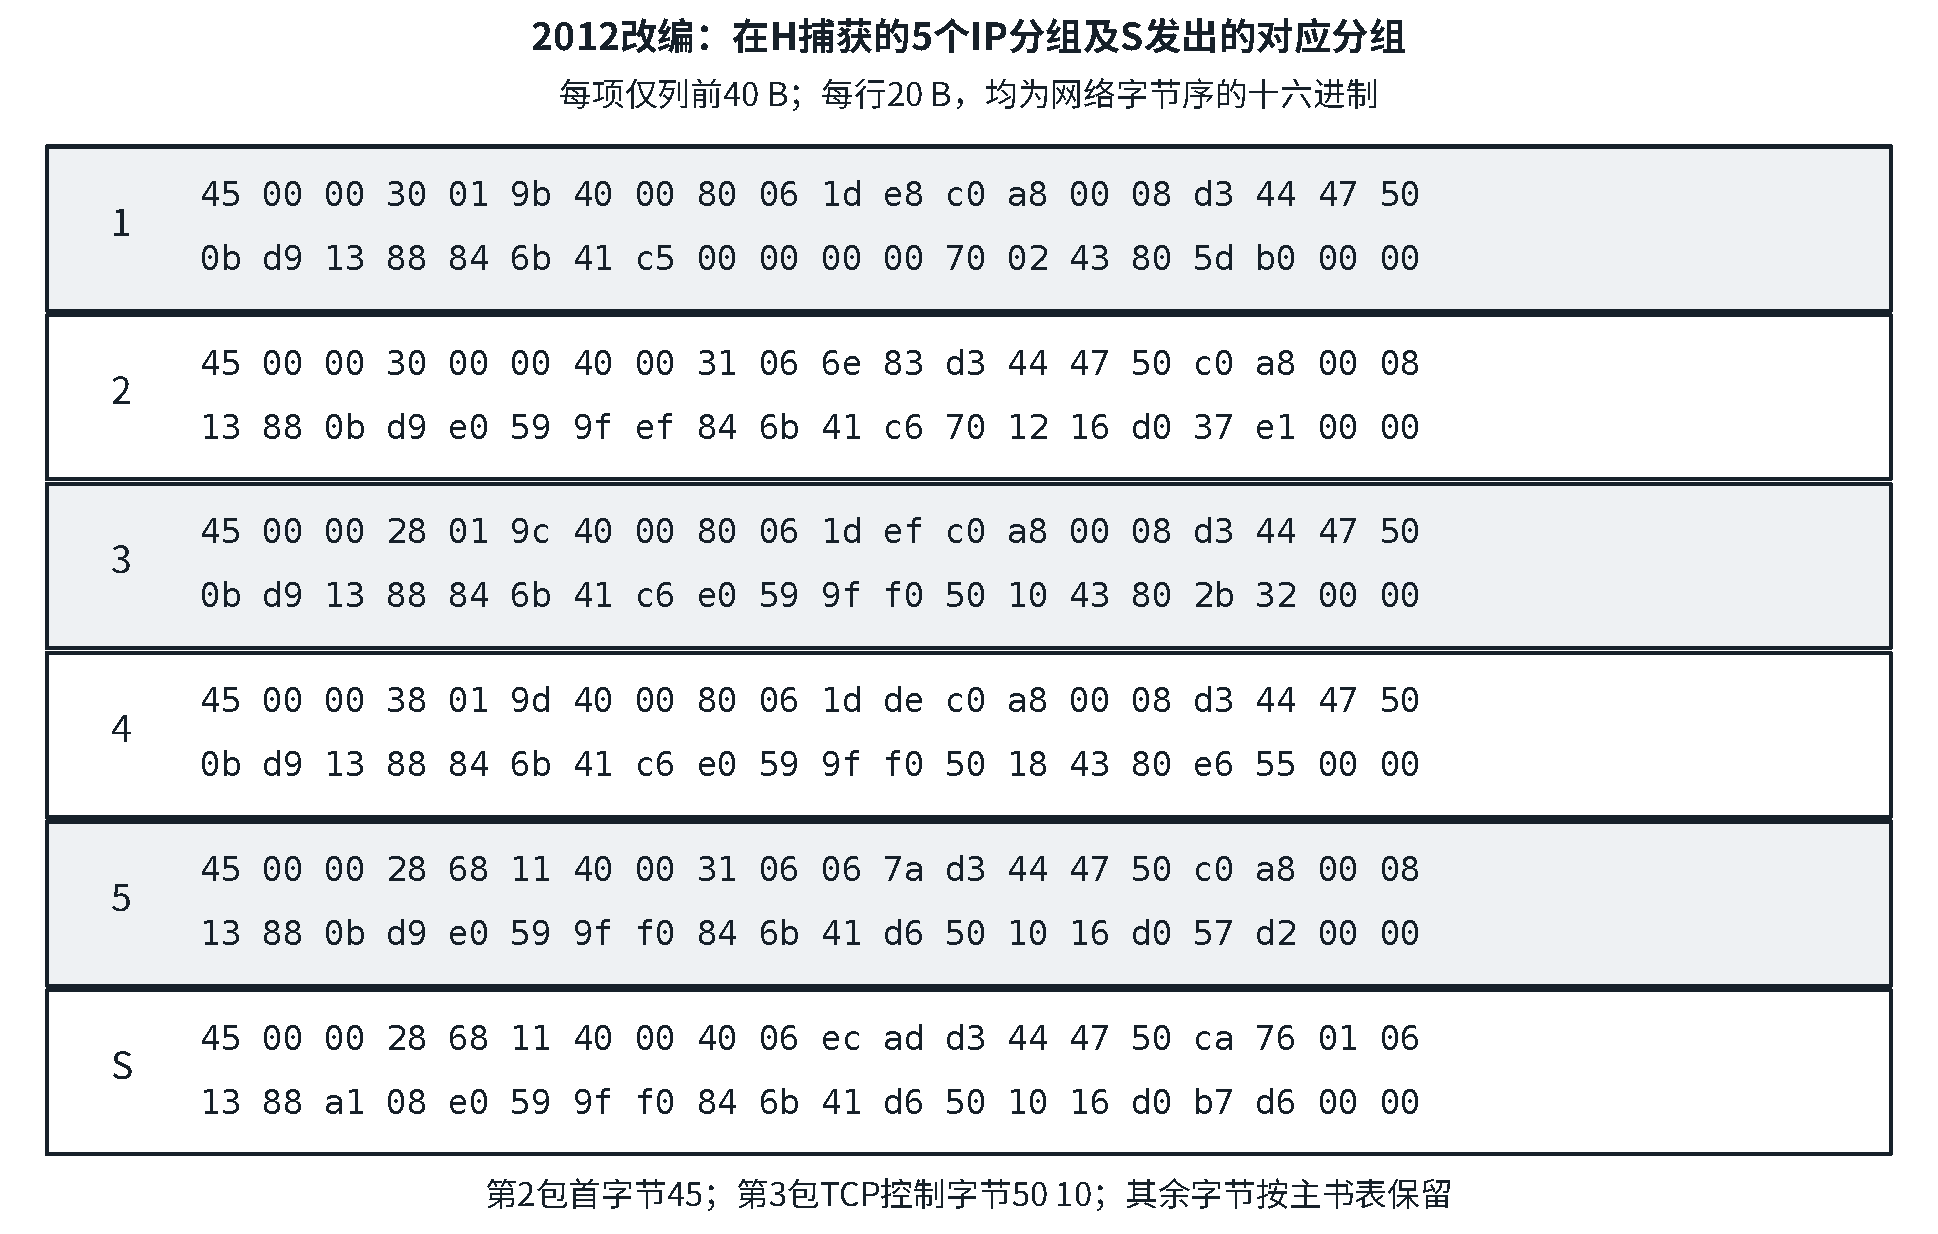
\includegraphics[width=\linewidth,height=108mm,keepaspectratio]{figures/CN25_packets_2012.pdf}
\caption{1～5为H处捕获的分组，S行为在服务器发出时捕获的对应分组；每行20 B}\label{cn-fig-packets2012}
\end{figure}

字段布局参照第4章IPv4首部格式和本章\hyperref[cn-fig-tcp-format]{TCP首部图}：IPv4源、目的地址分别位于第13～16、第17～20字节，TTL位于第9字节；IHL与TCP数据偏移字段均以4 B为单位。

（1）5个IP分组中，哪几个由H发送？哪几个完成TCP连接建立过程？哪几个在通过快速以太网传输时进行了填充？

（2）根据这5个IP分组，分析S已经收到的应用层数据有多少字节。

（3）若某个IP分组在S发出时的前40字节为图中S行，该IP分组到达H时经过了多少个路由器？

缓存只进不出时，累计接收量决定rwnd；每轮发送量同时受cwnd和剩余缓存限制。求零窗口时间须计至零窗口通告返回发送端；平均应用速率用总应用字节/题定时间，KB和kb/s分别按题设换算。

\par\medskip\Needspace{4\baselineskip}\noindent\hypertarget{CN05-E09}{}\label{CN05-E09}\textbf{例 5-9}\par\nobreak\smallskip

下图中H3访问Web服务器S。S为新建TCP连接分配20 KB（K=1024）接收缓存，MSS=1 KB，平均RTT=200 ms。H3建立连接时初始序号为100，持续按MSS大小发送数据，拥塞窗口初始阈值32 KB；S对收到的每个段确认并通告新接收窗口。连接建立后，S的TCP接收缓存只有数据存入、没有数据取出。图中R2的E0侧采用201.1.1.0/24。

\begin{figure}[H]
\centering
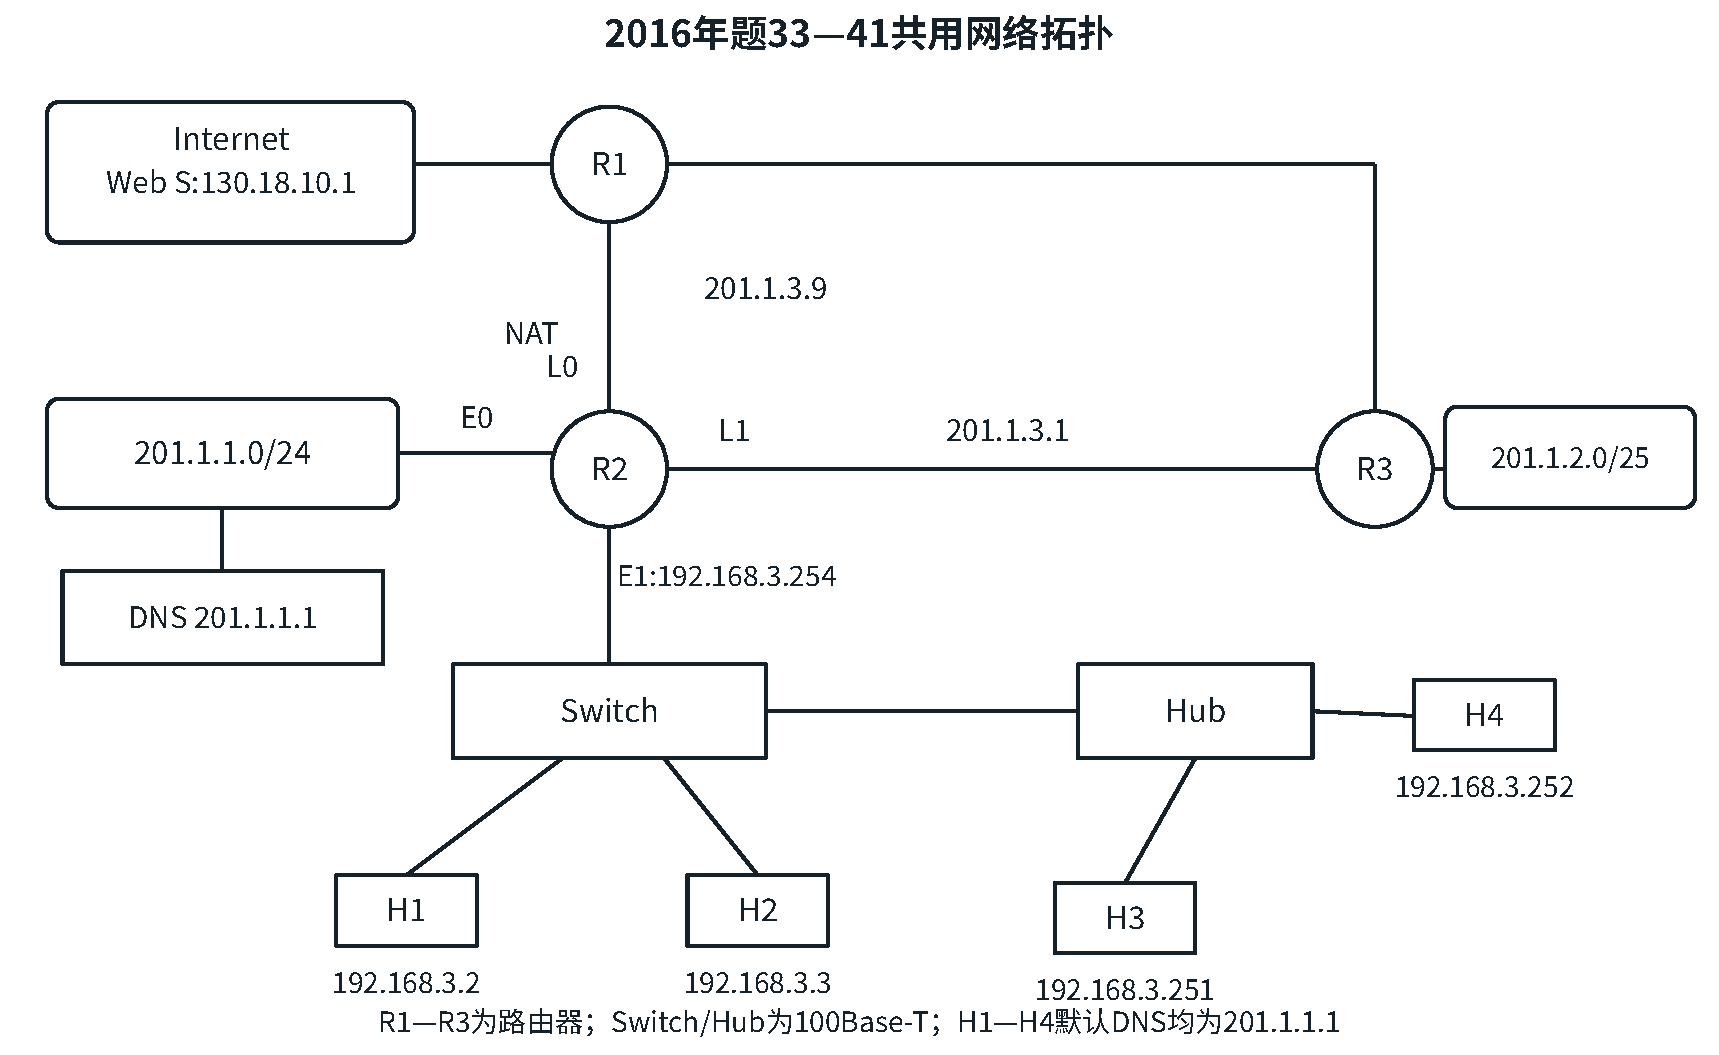
\includegraphics[width=\linewidth,height=108mm,keepaspectratio]{figures/CN14_dns_topology_2016.pdf}
\caption{H3为192.168.3.251，经Hub和R2访问130.18.10.1；复用2016年共用题图}\label{cn-fig-window2016}
\end{figure}

（1）连接建立时，H3收到的第二次握手TCP段的SYN、ACK标志位分别是多少？确认号是多少？

（2）H3收到的第8个确认段所通告的接收窗口是多少？此时拥塞窗口变为多少？发送窗口变为多少？

（3）发送窗口等于0时，下一个待发送的数据段序号是多少？从H3发送第1个数据段到发送窗口等于0，平均数据传输速率是多少？忽略段的传输时延。

（4）H3与S通信已结束，H3在\(t\)时刻请求断开连接。从\(t\)起，S释放该连接的最短时间是多少？
